\subsection{Generalization of Graph Heuristics}\label{subsec:generalization-of-graph-heuristics}

The first intuition behind NBFNet is that many of the traditional graph heuristics such as Katz-Index, Personalized PageRank~\cite{Page1998PageRank}
or Graph Distance can be generalized into a \textit{multiplication} and a \textit{summation} step.

\begin{figure}[h] % [h] attempts to place figure here, other options like [t]op, [b]ottom
    \centering % Centers the figure horizontally
    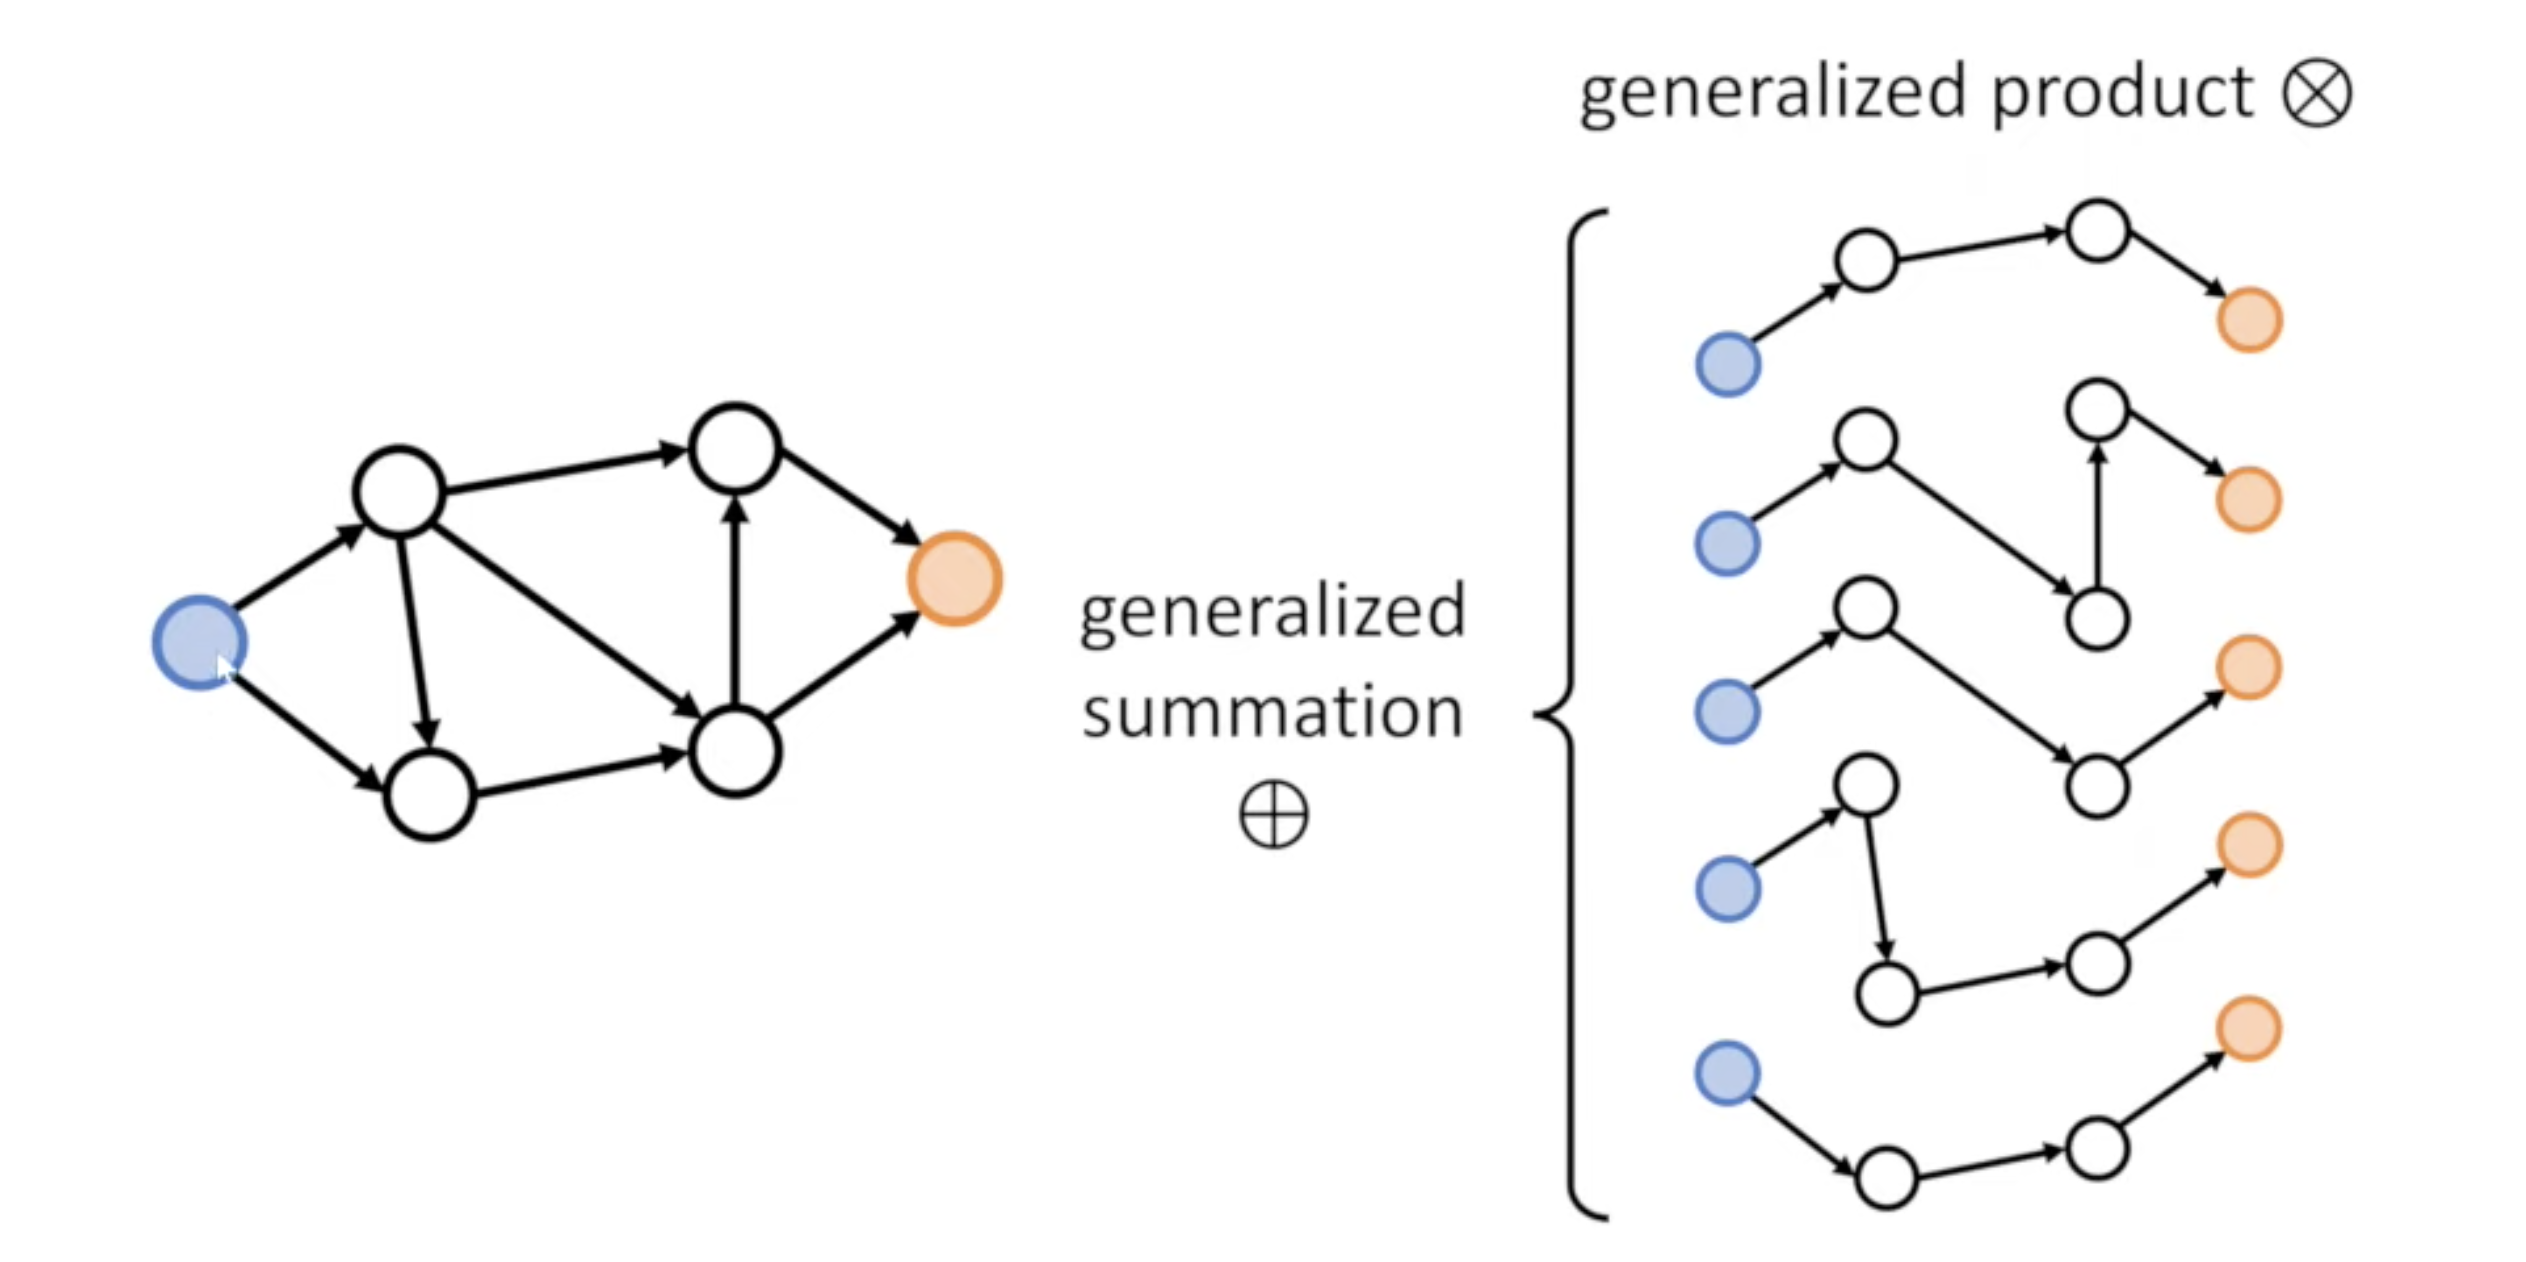
\includegraphics[width=0.8\linewidth]{figures/nbfnet-trad} % Include the image with desired width
    \caption{Generalized Graph Heuristic ~\cite{NBfnetPres}} % Add a caption
    \label{fig:nbfnet-trad} % Assign a label for referencing the figure in text
\end{figure}

For example, to find the shortest Graph Distance between two nodes, first we count the number of hops (generalized multiplication step by count) and then we select
the path with the fewest hop (generalized summation via the min function)

The second intuition behind NBFNet is that traditional link prediction methods that rely on encapsulating local neighborhoods~ ~\cite{RandomWalks, SubgraphExtraction}
perform random walks between the source and the target node.

Instead of these random walks, the pair representation can be formulated as "a generalized sum of path representations between u and v with a commutative
summation operator \bigoplus"~\cite{NBFNet}.

Within this summation, each path "is defined as a generalized product of the edge
representations in the path with the multiplication operator"~\cite{NBFNet}.

\subsection{Generalized Bellman-Ford Algorithm}\label{subsec:generalized-bellman-ford-algorithm}

Calculating such metrics for each node pair is computationally expensive due to its exponential nature.
As a solution, the NBFNet performs these calculations as part of a generalized Bellman-Ford algorithm, as that algorithm is highly
parallelizable (figure~\ref{fig:gen-bf}).

\begin{figure}[h] % [h] attempts to place figure here, other options like [t]op, [b]ottom
    \centering % Centers the figure horizontally
    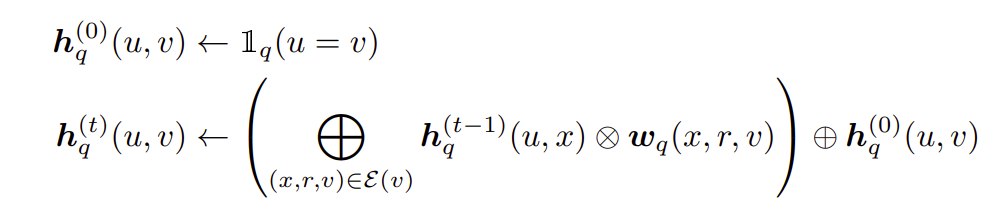
\includegraphics[width=0.8\linewidth]{figures/nbfnet-gen-bf} % Include the image with desired width
    \caption{Generalized Bellman-Ford Algorithm ~\cite{NBFNet}} % Add a caption
    \label{fig:gen-bf} % Assign a label for referencing the figure in text
\end{figure}

\subsection{Neural Bellman-Ford Networks}\label{subsec:neural-bellman-ford-networks}
Finally, to increase the potential of the models and detach from classical, handcrafted methods, the creators of NBFNet replaced
the generalized \textit{summation} and \textit{multiplication} operators with neural functions.

A Neural Bellman-Ford Network has three neural functions.

\subsubsection{The INDICATOR function}
"The INDICATOR function initializes a
representation on each node, which is
taken as the boundary condition of the generalized Bellman-Ford algorithm."~\cite{NBFNet}

It replaces the $\textbf{h}_q^{(0)}(u,v)\leftarrow\ \mathbbm{1}_q(u=v)$ step, seen on figure~\ref{fig:gen-bf}

\subsubsection{The MESSAGE function}
"The MESSAGE function replaces the binary multiplication operator \bigotimes"~\cite{NBFNet}


\subsubsection{The AGGREGATE function}
"The AGGREGATE function is a permutation invariant function
over sets that replaces the n-ary summation operator $\bigoplus$ \ldots
one may alternatively define AGGREGATE as the commutative binary operator $\bigoplus$ and apply it
to a sequence of messages." ~\cite{NBFNet}


The combination of the three neural function are shown on figure~\ref{fig:neural-bf}.

\begin{figure}[h] % [h] attempts to place figure here, other options like [t]op, [b]ottom
    \centering % Centers the figure horizontally
    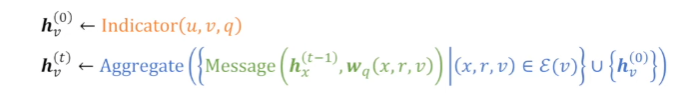
\includegraphics[width=0.65\linewidth]{figures/nbfnet-architecture} % Include the image with desired width
    \caption{Neural Bellman-Ford Network Architecture ~\cite{NBfnetPres}} % Add a caption
    \label{fig:neural-bf} % Assign a label for referencing the figure in text
\end{figure}


Finally, the learned vector representation is then fed into a multi-layer perceptron to predict the probability
of a tail node given a head node and a query relationship (figure~\ref{fig:nbfnet-mlp})

\begin{figure}[h] % [h] attempts to place figure here, other options like [t]op, [b]ottom
    \centering % Centers the figure horizontally
    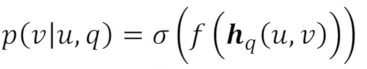
\includegraphics[width=0.4\linewidth]{figures/nbfnet-mlp} % Include the image with desired width
    \caption{Final Prediction Step in NBFNet ~\cite{NBfnetPres}} % Add a caption
    \label{fig:nbfnet-mlp} % Assign a label for referencing the figure in text
\end{figure}
